\documentclass[12pt, titlepage]{article}

\usepackage{fullpage}
\usepackage[round]{natbib}
\usepackage{multirow}
\usepackage{booktabs}
\usepackage{tabularx}
\usepackage{graphicx}
\usepackage{float}
\usepackage{hyperref}
\usepackage{xcolor}
\hypersetup{
    colorlinks,
    citecolor=black,
    filecolor=black,
    linkcolor=red,
    urlcolor=blue
}
\usepackage[round]{natbib}

\newcounter{acnum}
\newcommand{\actheacnum}{AC\theacnum}
\newcommand{\acref}[1]{AC\ref{#1}}

\newcounter{ucnum}
\newcommand{\uctheucnum}{UC\theucnum}
\newcommand{\uref}[1]{UC\ref{#1}}

\newcounter{mnum}
\newcommand{\mthemnum}{M\themnum}
\newcommand{\mref}[1]{M\ref{#1}}

\title{SE 3XA3: Module Guide\\Othello}

\author{Team \#2, JMS Corporation
		\\ Mohammed Mirajkar, mirajkam
		\\ Jinesh Patel, patelj60
		\\ Sankar Renganathan, renganas
}

\date{\today}

%\input{../../Comments}

\begin{document}

\maketitle

\pagenumbering{roman}
\tableofcontents
\listoftables
\listoffigures

\begin{table}[bp]
\caption{\bf Revision History}
\begin{tabularx}{\textwidth}{p{3cm}p{2cm}X}
\toprule {\bf Date} & {\bf Version} & {\bf Notes}\\
\midrule
06/11/2018 & 0.1 & Worked on Introduction and Behaviour Modules\\
06/11/2018 & 0.1 & Worked on Anticipated and Unlikely Changes as well as Module Hierachy\\
29/11/2018 & 1.0 & Revised Document\\
\bottomrule
\end{tabularx}
\end{table}

\newpage

\pagenumbering{arabic}

\section{Introduction}

{{\color{blue}JSM Corporation has implemented a web-based version of Othello that strives to provide a fresh new feel to playing the beloved board game. JSM Corporation has provided this module guide which contains information on the different modules that have been used to implement the game of Othello. The modules used in the project present a state of low coupling and high cohesion and this guide will run through how the project has been organized and how different functions interact with each other. This guide will touch on anticipated and unlikely changes, module decomposition, uses hierarchy and the tracability matrix to connect how each module depends on certain other modules. }


\section{Anticipated and Unlikely Changes} \label{SecChange}

This section lists possible changes to the system to help implement unfinished tasks or to improve the game.

\subsection{Anticipated Changes} \label{SecAchange}

Anticipated changes are the source of the information that is to be hidden
inside the modules. Ideally, changing one of the anticipated changes will only
require changing the one module that hides the associated decision. The approach
adapted here is called design for
change.

\begin{description}
\item[\refstepcounter{acnum} \actheacnum \label{acInput1}:] The algorithm for moves made by the AI.
\item[\refstepcounter{acnum} \actheacnum \label{acInput2}:] The animation time for valid moves .
\item[\refstepcounter{acnum} \actheacnum \label{acInput3}:] The animation time for invalid moves.
\item[\refstepcounter{acnum} \actheacnum \label{acInput4}:] The graphical user interface elements and format used to represent the game score.
\item[\refstepcounter{acnum} \actheacnum \label{acInput5}:] The storage method used to save and load the game state.
\end{description}

\subsection{Unlikely Changes} \label{SecUchange}

This sections lists changes that are not prioritized by the developers.

\begin{description}
\item[\refstepcounter{ucnum} \uctheucnum \label{ucIO}:] Input/Output devices
  (Input: File and/or Keyboard, Output: File, Memory, and/or Screen).
\item[\refstepcounter{ucnum} \uctheucnum \label{ucInput}:] The input data will always come via the user.
\item[\refstepcounter{ucnum} \uctheucnum \label{ucInput}:] The input format (will always be a click event).
\item[\refstepcounter{ucnum} \uctheucnum \label{ucInput}:] The algorithms for determining a valid and invalid move.
\item[\refstepcounter{ucnum} \uctheucnum \label{ucInput}:] The animations for making an invalid move and making a valid move.
\end{description}

\section{Module Hierarchy} \label{SecMH}

This section provides an overview of the module design. Modules are summarized
in a hierarchy decomposed by secrets in Table \ref{TblMH}. The modules listed
below, which are leaves in the hierarchy tree, are the modules that will
actually be implemented.

\begin{description}
\item [\refstepcounter{mnum} \mthemnum \label{mHH}:] Hardware-Hiding Module
\item [\refstepcounter{mnum} \mthemnum \label{mUI}:] Board Module
\item [\refstepcounter{mnum} \mthemnum \label{mVM}:] UI Module
\item [\refstepcounter{mnum} \mthemnum \label{mGM}:] Game Module
\item [\refstepcounter{mnum} \mthemnum \label{mGHM}:] Game History Module
\item [\refstepcounter{mnum} \mthemnum \label{mAM}:] AI Module
\end{description}


\begin{table}[h!]
\centering
\begin{tabular}{p{0.3\textwidth} p{0.6\textwidth}}
\toprule
\textbf{Level 1} & \textbf{Level 2}\\
\midrule

{None} & ~ \\
\midrule

\multirow{1}{0.3\textwidth}{Behaviour-Hiding Module} 
& {\color{blue}Board Module } Module\\
& {\color{blue}UI Module } Module\\
& Game Module\\
& Game History Module\\
\midrule

\multirow{1}{0.3\textwidth}{Software Decision Module} 
& AI Module\\
\bottomrule

\end{tabular}
\caption{Module Hierarchy}
\label{TblMH}
\end{table}

\section{Connection Between Requirements and Design} \label{SecConnection}

The design of the system is intended to satisfy the requirements developed in
the SRS. In this stage, the system is decomposed into modules. The connection
between requirements and modules is listed in Table \ref{TblRT}.

\section{Module Decomposition} \label{SecMD}

{\color{blue}
This section depicts how the project is organized into different modules and the main functionalities of the modules and how it contributes to the overall system}

\subsection{Hardware Hiding Modules (\mref{mHH})}

{\color{blue}
There is no hardware hiding module being implemented}


\subsection{Behaviour-Hiding Module}

\begin{description}
\item[Secrets:]The contents of the required behaviours.
\item[Services:]Includes programs that provide externally visible behaviour of
  the system as specified in the software requirements specification (SRS)
  documents. This module serves as a communication layer between the
  hardware-hiding module and the software decision module. The programs in this
  module will need to change if there are changes in the SRS.
\item[Implemented By:] --
\end{description}

\subsubsection{{\color{blue}Board Module }  (\mref{mUI})}

\begin{description}
\item[Secrets:]{\color{blue}Manages the state of the board } 
\item[Services:]Contains information of the state of the board and the validity of the board
\item[Implemented By:] HTML and JavaScript
\end{description}

\subsubsection{{\color{blue}UI Module } (\mref{mVM})}

\begin{description}
\item[Secrets:]{\color{blue}How the game responds to user input}
\item[Services:]Displays information and visuals in an organized manner to the user and reacts to input
\item[Implemented By:] HTML, JavaScript and CSS
\end{description}

\subsubsection{Game Module  (\mref{mGM})}

\begin{description}
\item[Secrets:]{\color{blue}How the game functions}
\item[Services:]Calculates moves and score and checks the validity of the move
\item[Implemented By:] JavaScript
\end{description}

\subsubsection{Game History Module  (\mref{mGHM})}

\begin{description}
\item[Secrets:]{\color{blue}Helps keep track of the past states of the game}
\item[Services:]Stores the past states of the game board to be accessed later
\item[Implemented By:] JavaScript
\end{description}


\subsection{Software Decision Module  (\mref{mAM})}

\begin{description}
\item[Secrets:] The design decision based on mathematical theorems, physical
  facts, or programming considerations. The secrets of this module are
  \emph{not} described in the SRS.
\item[Services:] Includes data structure and algorithms used in the system that
  do not provide direct interaction with the user. 
  % Changes in these modules are more likely to be motivated by a desire to
  % improve performance than by externally imposed changes.
\item[Implemented By:] --
\end{description}

\subsubsection{AI Modules}

\begin{description}
\item[Secrets:]The AI Controller
\item[Services:]Chooses moves based on the state of the board in a time efficient manner
\item[Implemented By:] JavaScript
\end{description}

\section{Traceability Matrix} \label{SecTM}

This section shows two traceability matrices: between the modules and the
requirements and between the modules and the anticipated changes.

% the table should use mref, the requirements should be named, use something
% like fref
\begin{table}[htp]
\centering
\begin{tabular}{p{0.2\textwidth} p{0.6\textwidth}}
\toprule
\textbf{Req.} & \textbf{Modules}\\
\midrule
FR1 & \mref{mVM}, \mref{mUI}\\
FR2 & \mref{mVM}, \mref{mGM}\\
FR3 & \mref{mVM}, \mref{mUI}\\
FR4 & \mref{mGM}, \mref{mAM}\\
FR5 & \mref{mVM}, \mref{mGM}, \mref{mUI}\\
FR6 & \mref{mGM}, \mref{mVM}\\
FR7 & \mref{mGM}, \mref{mUI}, \mref{mVM}\\
FR8 & \mref{mGM}, \mref{mUI}, \mref{mGHM} \\
FR9 & \mref{mGM}, \mref{mUI}, \mref{mGHM} \\
NF1 & \mref{mVM}\\
NF2 & \mref{mVM}\\
NF3 & \mref{mVM}\\
NF4 & \mref{mVM}\\
NF5 & \mref{mVM}\\
NF6 & \mref{mVM}\\
NF7 & \mref{mVM}\\
NF8 & \mref{mVM}, \mref{mAM}\\
NF9 & \mref{mVM}, \mref{mGM}, \mref{mUI} \\
NF10& \mref{mVM}, \mref{mGM}, \mref{mUI} \\
NF11 & \mref{mGM} \\
NF12 & \mref{mGM} \\
NF13 &   N/A\\
NF14 &\mref{mGHM}\\
NF15&\mref{mGHM}\\
NF16 &   N/A\\

\bottomrule
\end{tabular}
\caption{Trace Between Requirements and Modules}
\label{TblRT}
\end{table}

\begin{table}[H]
\centering
\begin{tabular}{p{0.2\textwidth} p{0.6\textwidth}}
\toprule
\textbf{AC} & \textbf{Modules}\\
\midrule
\acref{acInput1} & \mref{mAM}\\
\acref{acInput2} & \mref{mVM}\\
\acref{acInput3} & \mref{mVM}\\
\acref{acInput4} & \mref{mVM}\\
\acref{acInput5} & \mref{mGM}\\
\bottomrule
\end{tabular}
\caption{Trace Between Anticipated Changes and Modules}
\label{TblACT}
\end{table}

\section{Use Hierarchy Between Modules} \label{SecUse}

{\color{blue}
This section shows the relationship of each module, identifying leaf modules as well as the heirarchy of the modules. A DAG is used to portray this in order to show the which module use other modules and which modules are used by other modules}.

This references \citet{Parnas1978}, and Figure \ref{FigUH}

\begin{figure}[H]
\centering
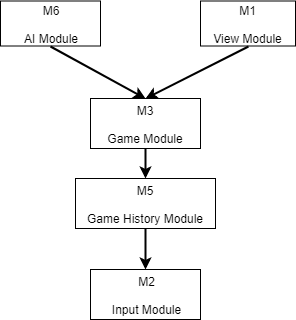
\includegraphics[width=0.8\textwidth]{UsesHierarchy3.png}
\caption{Use hierarchy among modules}
\label{FigUH}
\end{figure}

\section{Project Schedule}

The project schedule is layed out by this \href{https://gitlab.cas.mcmaster.ca/patelj60/3XA3-G02-Othello/blob/master/ProjectSchedule/3XA3_Project_Plan.pdf}{Gantt Chart} created by JSM Corp.

%\section*{References}

\bibliographystyle {plainnat}
\bibliography {MG}

\end{document}
